\documentclass[a4paper,12pt]{paper}
\usepackage{mycommands}


\title{Lecture 22: Free Oscillations}
\author{David Al-Attar \\ Michaelmas Term, \the\year}

\begin{document}

\maketitle

\section*{Outline and Motivation}

Having obtained the equations of motion for a self-gravitating earth model, we begin our study of the Earth's 
free oscillations or normal modes (the terms are synonymous). The starting point is developing a concise operator 
notation that closely resembles what you know from quantum mechanics. We analyse the associated eigenvalue problem in a 
non-rotating earth model, with the mathematics again being near identical to that in quantum physics. In particular, 
the forced response of such an earth model is obtained as an eigenfunction expansion, with the frequency-domain 
response having resonances at each of the eigenfrequencies. It is due to this fact that the observations of the 
eigenfrequencies can be made from sufficiently long time-series, with these data providing important constraints on 
Earth structure. Indeed, such frequencies form the principal constraint on the Earth's density. 

\section*{Linearised equations of motion}

Within Lecture 20 we obtained the following linearised equations of motion
\begin{equation}
\rho\left(\frac{\partial^{2}u_{i}}{\partial t^{2}}+2\epsilon_{ijk}\Omega_{j}\frac{\partial u_{k}}{\partial t}
+\epsilon_{ijk}\epsilon_{klm}\Omega_{j}\Omega_{l}u_{m}\right)-\frac{\partial}{\partial x_{j}}\left(A_{ijkl}\frac{\partial u_{k}}{\partial x_{l}}\right)
-\rho\gamma_{i}^{1}=-\frac{\partial\overline{S}_{ij}}{\partial x_{j}},
\end{equation}
for a self-gravitating and rotating elastic earth model relative to a co-rotating reference frame. Here $\rho$ is the equilibrium density, $u_{i}$ the displacement vector, $\Omega_{i}$ is the angular velocity, $A_{ijkl}$ the elastic tensor, $\gamma_{i}^{1}$ the perturbation to the gravitational acceleration which is given concretely by
\begin{equation}
\gamma_{i}^{1}=-G\int_{M}\rho'\left(\frac{\delta_{ij}}{[(x_{k}-x_{k}')(x_{k}-x_{k}')]^{3/2}}-\frac{3(x_{i}-x_{i}')(x_{j}-x_{j}')}{[(x_{k}-x_{k}')(x_{k}-x_{k}')]^{5/2}}\right)(u_{j}-u_{j}')\dd^{3}\mathbf{x}',
\end{equation}
where it is understood that primed terms are functions of the integration variable, and finally $\overline{S}_{ij}$ is the stress glut associated with a seismic source. The boundary conditions for the problem are
\begin{equation}
A_{ijkl}\frac{\partial u_{k}}{\partial x_{l}}\hat{n}_{j}=\overline{S}_{ij}\hat{n}_{j}
\end{equation}
on $\partial M$. While these equations express quite simple physics, they do have a complicated form, and hence it will help things greatly to find a simpler notation.

As a first step to doing this, we will express the equations in what is known as the weak form. Letting $w_{i}$ be an arbitrary function we find from eq.(1) that
\begin{equation}
\int_{M}\left[\rho\left(\frac{\partial^{2}u_{i}}{\partial t^{2}}+2\epsilon_{ijk}\Omega_{j}\frac{\partial u_{k}}{\partial t}+\epsilon_{ijk}\epsilon_{klm}\Omega_{j}\Omega_{l}u_{m}\right)-\frac{\partial}{\partial x_{j}}(A_{ijkl}\frac{\partial u_{k}}{\partial x_{l}}-\overline{S}_{ij})-\rho\gamma_{i}^{1}\right]w_{i}^{*}\dd^{3}\mathbf{x}=0.
\end{equation}
where we note that $\mathbf{w}$ has been allowed to be complex-valued and $^*$ denotes a complex conjugate\footnote{The reason for this generality is that later we will consider an associated eigenvalue problem, and in this context complex-valued fields naturally occur.}. Performing an integration by parts and using the boundary conditions this becomes
\begin{equation}
\int_{M}\left[\rho\left(\frac{\partial^{2}u_{i}}{\partial t^{2}}+2\epsilon_{ijk}\Omega_{j}\frac{\partial u_{k}}{\partial t}+\epsilon_{ijk}\epsilon_{klm}\Omega_{j}\Omega_{l}u_{m}-\gamma_{i}^{1}\right)w_{i}^{*}+(A_{ijkl}\frac{\partial u_{k}}{\partial x_{l}}-\overline{S}_{ij})\frac{\partial w_{i}^{*}}{\partial x_{j}}\right]\dd^{3}\mathbf{x}=0.
\end{equation}
We have obtained this result for arbitrary $\mathbf{w}$ whenever $\mathbf{u}$ satisfies eq. (1) and (3). Conversely, the argument can be reversed to show that if eq.(5) holds for all $\mathbf{w}$, then the field $\mathbf{u}$ must satisfy eq.(1) and (3), this being the weak form of the problem.

Eq.(5) involves several terms that depend linearly on $\mathbf{u}$ and conjugate-linearly on $\mathbf{w}$, with such objects known as a sesquilinear forms\footnote{The term "sesqui" is used instead of "bilinear" to indicate that the form is linear in one argument and conjugate linear in the other.}. For example, if we define
\begin{equation}
\langle \mathbf{w}|P|\mathbf{u}\rangle=\int_{M}\rho w_{i}^{*}u_{i}\dd^{3}\mathbf{x},
\end{equation}
then we can write the acceleration term in the weak form as
\begin{equation}
\langle \mathbf{w}|P|\ddot{\mathbf{u}}\rangle.
\end{equation}
where time-derivatives are denoted using dots. Hopefully the notation here should remind you of bra-ket notation. We will call $\langle \mathbf{w}|P|\mathbf{u}\rangle$ the kinetic energy form, and note that it may be associated with an operator P that acts on displacement vectors by $(P\mathbf{u})_{i}=\rho u_{i}$. In a similar manner we define
\begin{equation}
\langle \mathbf{w}|W|\mathbf{u}\rangle=\int_{M}2\rho\epsilon_{ijk}w_{i}^{*}\Omega_{j}u_{k}\dd^{3}\mathbf{x}
\end{equation}
which we call the Coriolis form, this being associated with an operator W defined by $(W\mathbf{u})_{i}=2\rho\epsilon_{ijk}\Omega_{j}u_{k}$. We finally have the potential energy form
\begin{equation}
\langle \mathbf{w}|H|\mathbf{u}\rangle=\int_{M}\left(\rho\epsilon_{ijk}\epsilon_{klm}w_{i}^{*}\Omega_{j}\Omega_{l}u_{m}+A_{ijkl}\frac{\partial w_{i}^{*}}{\partial x_{j}}\frac{\partial u_{k}}{\partial x_{l}}-\rho w_{i}^{*}\gamma_{i}^{1}\right)\dd^{3}\mathbf{x},
\end{equation}
and write the force term as
\begin{equation}
\langle \mathbf{w}|\mathbf{f}\rangle=\int_{M}\overline{S}_{ij}\frac{\partial w_{i}^{*}}{\partial x_{j}}\dd^{3}\mathbf{x}.
\end{equation}
In this manner, we can concisely express the weak form of the equations of motion as
\begin{equation}
\langle \mathbf{w}|P|\ddot{\mathbf{u}}\rangle+\langle \mathbf{w}|W|\dot{\mathbf{u}}\rangle+\langle \mathbf{w}|H|\mathbf{u}\rangle=\langle \mathbf{w}|\mathbf{f}\rangle,
\end{equation}
which is to hold for all test functions $\mathbf{w}$. From this equation it would be very tempting to write the problem in operator form as
\begin{equation}
P\ddot{\mathbf{u}}+W\dot{\mathbf{u}}+H\mathbf{u}=\mathbf{f}.
\end{equation}
Here it is, however, important to remember that the problem's boundary conditions are incorporated within the potential energy form and force term. As a result, we should see eq.(12) as only a formal notation; the weak form incorporates the boundary conditions directly, and is generally to be preferred.

\subsection*{Properties of the sesquilinear forms}
If we look at the kinetic energy form, then it is clear that
\begin{equation}
\langle \mathbf{w}|P|\mathbf{u}\rangle=\langle \mathbf{u}|P|\mathbf{w}\rangle^{*},
\end{equation}
and we say that the form is self-adjoint. Equivalently we can say that the associated operator P is self-adjoint. We also note that $\langle \mathbf{u}|P|\mathbf{u}\rangle$ is positive for any non-zero vector field $\mathbf{u}$, and hence the kinetic energy form defines an inner product. In contrast, for the Coriolis form, we find that
\begin{equation}
\langle \mathbf{w}|W|\mathbf{u}\rangle=\int_{M}2\rho\epsilon_{ijk}w_{i}^{*}\Omega_{j}u_{k}\dd^{3}\mathbf{x} = -\left(\int_{M}2\rho\epsilon_{ijk}u_{i}^{*}\Omega_{j}w_{k}\dd^{3}\mathbf{x}\right)^{*} = -\langle \mathbf{u}|W|\mathbf{w}\rangle^{*},
\end{equation}
this meaning that it is anti self-adjoint. This implies, in particular, that $\langle \mathbf{u}|W|\mathbf{u}\rangle$ is purely imaginary for any $\mathbf{u}$, while it vanishes if the field has real components.

For the potential energy form it is readily checked that the term associated with elasticity is self-adjoint due to the hyperelastic symmetry $A_{ijkl}=A_{klij}$. Similarly for the centrifugal term we have
\begin{equation}
\int_{M}\rho\epsilon_{ijk}\epsilon_{klm}w_{i}^{*}\Omega_{j}\Omega_{l}u_{m}\dd^{3}\mathbf{x}=\left(\int_{M}\rho\epsilon_{ijk}\epsilon_{klm}w_{i}\Omega_{j}\Omega_{l}u_{m}^{*}\dd^{3}\mathbf{x}\right)^{*} = \left(\int_{M}\rho\epsilon_{ijk}\epsilon_{klm}u_{i}^{*}\Omega_{j}\Omega_{l}w_{m}\dd^{3}\mathbf{x}\right)^{*},
\end{equation}
where to obtain the final equality we have just relabelled and permuted the indices appropriately. What takes more work is to show that
\begin{equation}
\int\rho w_{i}^{*}\gamma_{i}^{1}(\mathbf{u})\dd^{3}\mathbf{x}=\int\rho\gamma_{i}^{1}(\mathbf{w})^{*}u_{i}\dd^{3}\mathbf{x}.
\end{equation}
where we have included arguments to show which displacement vector the gravitational acceleration term corresponds to. Proof of this identity not difficult but nor is it enlightening. The end result is that the potential energy form is also self-adjoint.

\subsection*{Eigenfunctions and eigenvalues in a non-rotating earth model}
Recall from the scaling arguments in Lecture 20 that while self-gravitation is important for low frequency seismology, rotation remains only a relatively small effect. For the moment let us, therefore, suppose that the earth model is non-rotating. The equations of motion then read in weak form
\begin{equation}
\langle \mathbf{w}|P|\ddot{\mathbf{u}}\rangle+\langle \mathbf{w}|H|\mathbf{u}\rangle=\langle \mathbf{w}|\mathbf{f}\rangle,
\end{equation}
which is to hold for any $\mathbf{w}$, and where it is understood that the centrifugal contribution to the potential energy form has been removed. Suppose first that we set the stress glut equal to zero, and consider a time-harmonic displacement field
\begin{equation}
u_{i}(\mathbf{x},t)=s_{i}(\mathbf{x})e^{i\omega t}
\end{equation}
with $\mathbf{s}$ the spatial part of the solution, and $\omega$ an angular frequency. Putting this into eq. (17) we arrive at
\begin{equation}
-\omega^{2}\langle \mathbf{w}|P|\mathbf{s}\rangle+\langle \mathbf{w}|H|\mathbf{s}\rangle=0.
\end{equation}
This equation has the trivial solution $\mathbf{s}=0$ but it is interesting to ask whether it has any non-trivial solutions. As you no doubt recognise, this is an eigenvalue problem with $\mathbf{s}$ the eigenfunction and $\omega$ the eigenfrequency. Note, in particular, that the boundary conditions for the problem are built into the weak form of the equations of motion, and hence these eigenfunctions satisfy traction-free boundary conditions on $\partial M$.

Due to the self-adjointness of the kinetic and potential energy forms, we can quickly establish some expected properties of the eigenfunctions and eigenfrequencies. Let $\mathbf{s}_{1}$ be an eigenfunction associated with eigenfrequency $\omega_{1}$, and $\mathbf{s}_{2}$ an eigenfunction associated with eigenfrequency $\omega_{2}$. By definition we then have
\begin{equation}
-\omega_{1}^{2}\langle \mathbf{w}|P|\mathbf{s}_{1}\rangle+\langle \mathbf{w}|H|\mathbf{s}_{1}\rangle=0,
\end{equation}
for any $\mathbf{w}$. Taking this test function equal to $\mathbf{s}_{2}$, and using the self-adjointness of the forms, it follows that
\begin{equation}
0=-\omega_{1}^{2}\langle \mathbf{s}_{2}|P|\mathbf{s}_{1}\rangle+\langle \mathbf{s}_{2}|H|\mathbf{s}_{1}\rangle=-\omega_{1}^{2}\langle \mathbf{s}_{1}|P|\mathbf{s}_{2}\rangle^{*}+\langle \mathbf{s}_{1}|H|\mathbf{s}_{2}\rangle^{*}.
\end{equation}
Using the eigenvalue equation for $\mathbf{s}_{2}$ we know that
\begin{equation}
\langle \mathbf{s}_{1}|H|\mathbf{s}_{2}\rangle=\omega_{2}^{2}\langle \mathbf{s}_{1}|P|\mathbf{s}_{2}\rangle,
\end{equation}
and hence from eq. (21) we have shown that
\begin{equation}
(\omega_{1}^{2}-\omega_{2}^{2*})\langle \mathbf{s}_{1}|P|\mathbf{s}_{2}\rangle^{*}=0 .
\end{equation}
Taking $\mathbf{s}_{1}=\mathbf{s}_{2}$, and recalling that $\langle \mathbf{u}|P|\mathbf{u}\rangle$ is positive for any non-zero displacement field, we conclude that $\omega_{1}^{2*}=\omega_{1}^{2}$, which is to say that the squared-eigenfrequencies are real. Next, if we suppose that $\omega_{1}\ne\omega_{2}$, then we must have
\begin{equation}
\langle \mathbf{s}_{1}|P|\mathbf{s}_{2}\rangle=0
\end{equation}
this meaning that eigenfunctions with different squared-eigenfrequencies are orthogonal relative to the inner product defined by kinetic energy form. Orthogonality relative to such a "mass weighted" inner product should be familiar from your prior study of linear oscillations of finite-dimensional mechanical systems.

The following additional properties of these eigenfunctions and eigenfrequencies will be stated without proof\footnote{The validity 
of these results in solid earth models can be established rigorously based on the theory of elliptic partial differential operators. 
Their proof, and indeed general validity, within models containing in-viscid fluid regions like the outer core remains an open problem.}:
\begin{enumerate}
    \item Each squared-eigenfrequency is associated with a finite-dimensional eigenspace.  Eigenfunctions within the same eigenspace need not be orthogonal, but we can always select a basis such that they are.
    \item There is a countable infinity of squared-eigenfrequencies. Their values are bounded from below, and accumulate only at infinity. 
    The latter point means that in a finite-interval there can only be a finite number of squared-eigenfrequencies.
    \item The eigenfunctions form a complete orthonormal basis for vector fields in the earth model. This means that an arbitrary vector 
    field can be expressed as a convergent sum of the eigenfunctions, with the necessary expansion coefficients readily determined due to 
    their orthogonality.
\end{enumerate}
To proceed, we let $k=0,...,\infty$ label the different squared eigenfrequencies, $\omega_{k}^{2}$. For each $k$, there is then a 
finite-dimensional eigenspace, and we use a second index $m$ to label the elements of its basis. Note that the range of $m$ can 
vary with $k$, but we leave this implicit within the notation. The $m$th eigenfunction belonging to the $k$th eigenspace will be 
written $|km\rangle$ in a manner familiar from quantum mechanics. These eigenfunctions can be orthonormalised relative to the kinetic 
energy form, this meaning that
\begin{equation}
\langle km|P|k'm'\rangle=\delta_{kk'}\delta_{mm'},
\end{equation}
for all possible indices. Using this notation, we can then express the completeness of the eigenfunctions by noting that a displacement 
field $\mathbf{u}$ can be expanded as
\begin{equation}
\mathbf{u}=\sum_{km}\langle km|P|\mathbf{u}\rangle|km\rangle ,
\end{equation}
where $\langle km|P|\mathbf{u}\rangle$ are the expansion coefficients of the $(k,m)$th term.

\subsection*{Eigenfunction expansions}

\begin{figure}[h]
\centering
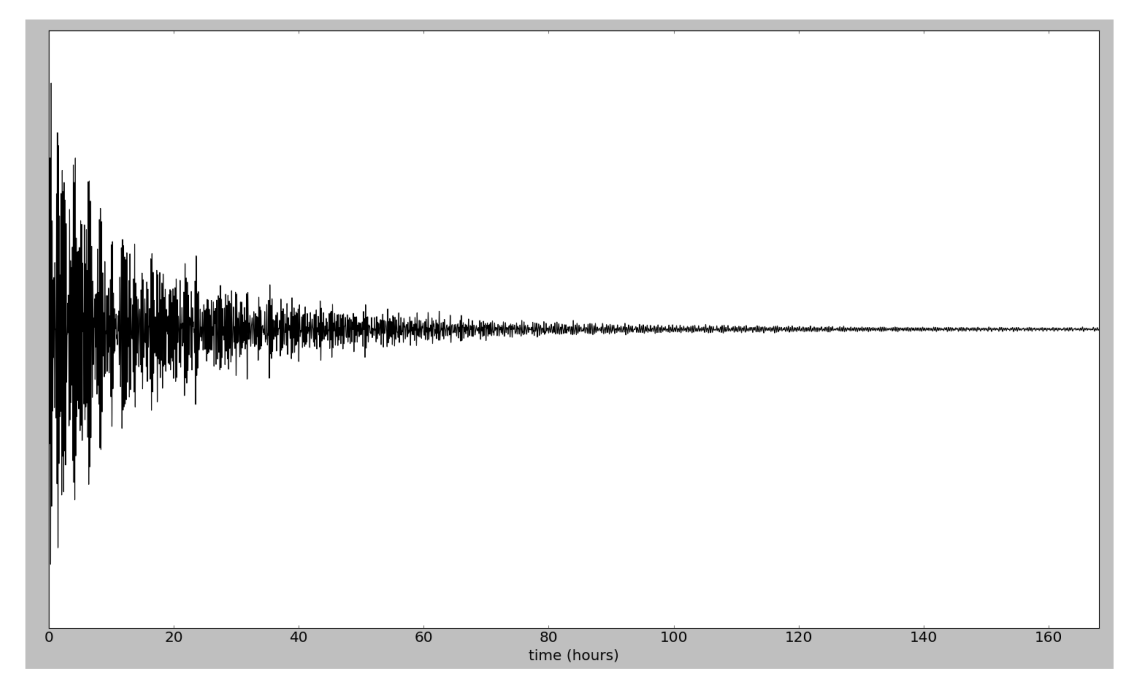
\includegraphics[width=\textwidth]{figures/L11F1.png}
\caption{A seven day long vertical component seismogram following the a magnitude 8.2
earthquake in Bolivia in 1994. Note also that the overall amplitude decays in a
roughly exponential fashion. This is due to attenuation within the Earth, but we
ignore this effect within our current discussion.}
\label{fig:fig1}
\end{figure}

Recall that the equations of motion in weak form are given by
\begin{equation}
\langle \mathbf{w}|P|\ddot{\mathbf{u}}\rangle+\langle \mathbf{w}|H|\mathbf{u}\rangle=\langle \mathbf{w}|\mathbf{f}\rangle,
\end{equation}
for any test-function $\mathbf{w}$. These equations can be usefully studied in the frequency-domain, where we use the convention
\begin{equation}
\tilde{\mathbf{u}}(\mathbf{x},\omega)=\int_{0}^{\infty}\mathbf{u}(\mathbf{x},t)e^{-i\omega t}dt, \quad \mathbf{u}(\mathbf{x},t)=\frac{1}{2\pi}\int_{-\infty}^{\infty}\tilde{\mathbf{u}}(\mathbf{x},\omega)e^{i\omega t}dt.
\end{equation}
noting that the initial conditions that $\mathbf{u}$ and $\dot{\mathbf{u}}$ vanish before time $t=0$ has been built into the forward transformation. It is readily seen that the Fourier transformed equations of motion take the form
\begin{equation}
-\omega^{2}\langle \mathbf{w}|P|\tilde{\mathbf{u}}\rangle+\langle \mathbf{w}|H|\tilde{\mathbf{u}}\rangle=\langle \mathbf{w}|\tilde{\mathbf{f}}\rangle.
\end{equation}
Using the completeness of the eigenfunctions, we know that we can write
\begin{equation}
\tilde{\mathbf{u}}=\sum_{k'm'}\langle k'm'|P|\tilde{\mathbf{u}}\rangle|k'm'\rangle ,
\end{equation}
for some frequency-dependent coefficients, $\langle k'm'|P|\tilde{\mathbf{u}}\rangle$, that are to be determined. Putting this eigenfunction expansion into eq. (29) we find
\begin{equation}
\sum_{k'm'}[-\omega^{2}\langle \mathbf{w}|P|k'm'\rangle+\langle \mathbf{w}|H|k'm'\rangle]\langle k'm'|P|\tilde{\mathbf{u}}\rangle=\langle \mathbf{w}|\tilde{\mathbf{f}}\rangle.
\end{equation}
which can be simplified using the eigenvalue problem satisfied by $|k'm'\rangle$ to read
\begin{equation}
\sum_{k'm'}(-\omega^{2}+\omega_{k'}^{2})\langle \mathbf{w}|P|k'm'\rangle\langle k'm'|P|\tilde{\mathbf{u}}\rangle=\langle \mathbf{w}|\tilde{\mathbf{f}}\rangle .
\end{equation}
Finally, we take the test function equal to $|km\rangle$, and use the orthonormality condition in eq.(25) to find that the $(k,m)$th coefficient of $\tilde{\mathbf{u}}$ is given by
\begin{equation}
\langle km|P|\tilde{\mathbf{u}}\rangle=\frac{\langle km|\tilde{\mathbf{f}}\rangle}{\omega_{k}^{2}-\omega^{2}}
\end{equation}
In this manner, we have obtained the eigenfunction expansion solution
\begin{equation}
\tilde{\mathbf{u}}=\sum_{km}\frac{\langle km|\tilde{\mathbf{f}}\rangle}{\omega_{k}^{2}-\omega^{2}}|km\rangle ,
\end{equation}
for the frequency-domain problem. Within the second problem set you can, in an optional question, obtain the corresponding time-domain solution by inversion of the Fourier transform using contour integration. For those unfamiliar with such methods, it will be sufficient to verify that the given solution does work through direct substitution.


\begin{figure}[h]
\centering
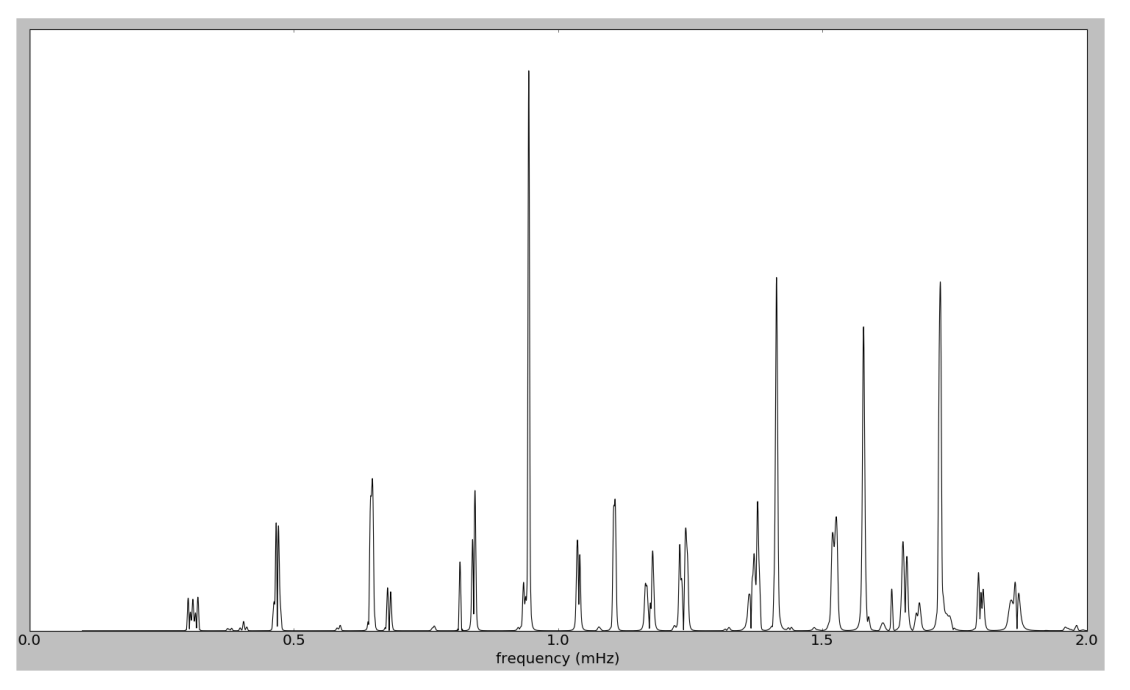
\includegraphics[width=\textwidth]{figures/L11F2.png}
\caption{The amplitude spectra corresponding to Fig. 1. In some cases individual mode
peaks can be identified, but especially at higher-frequencies there is substantial
overlap of the peaks due both to attenuation and an insufficiently long time series.}
\label{fig:fig2}
\end{figure}

Looking at eq. (34), it is notable that there are singularities at $\pm\omega_{k}$ for each k. Supposing for the moment
 that the squared-eigenfrequencies are all positive, these singularities lie along the real line. Physically, we are seeing
  resonances in the frequency-domain response when the system is driven at one of its eigenfrequencies. From an actual seismic 
  record we could take its Fourier transform, look for associated resonance peaks, and hence measure some of the eigenfrequencies 
  of the Earth. Note that these frequencies are determined solely by Earth structure, and hence their measurement provides a possible
   means to avoid the source-structure trade-off that is ever present in seismology.

To consider such measurements further, it is important to note that recorded seismograms are not of an infinite length, and so their Fourier transform will not yield eq. (34) exactly. In fact, within a more complete treatment there is also slight attenuation that shifts the singularities into the upper half-plane. To understand what happens with a finite-length time series, we can introduce a windowing function, $h(t)$, that is non-zero only in the range $[0,T]$, and so write the observed time-series as
\begin{equation}
\mathbf{u}_{obs}(t)=h(t)\mathbf{u}(t)
\end{equation}
where we neglect spatial arguments for simplicity. Taking the Fourier transform of such a time-series and applying the convolution theorem we find
\begin{equation}
\tilde{\mathbf{u}}_{obs}(\omega)\propto\int_{-\infty}^{\infty}\tilde{\mathbf{u}}(\omega')\tilde{h}(\omega'-\omega)d\omega',
\end{equation}
with the right hand side being proportional to the convolution of the two Fourier transforms. The end result is that the singularities of the Fourier-domain solution in eq. (34) are smoothed out within real observations. The extent of the smoothing is controlled primarily by the length of the time-series, with the support of $\tilde{h}$ being largely confined to an interval whose width scales like $T^{-1}$. This is, of course, a familiar result; longer time-series provide better resolution in the frequency-domain. It is for this reason that observational work on the Earth's free oscillations is concerned only with the largest earthquakes, the response to which can remain above background noise for many days. Even so, within observed spectra we cannot always identify individual mode peaks, and this is especially true in cases of near degeneracy that we will examine in more detail in the next lecture.

\subsection*{Gravitational stability}
Within the previous section we assumed that the squared eigenfrequencies were all positive, with the result that each term in the mode sum is associated with two simple poles on the real axis, and hence oscillatory contributions to the time-domain solution. If, instead, a squared eigenfrequency, $\omega_{k}^{2}$, was negative then there would be two simple poles on the imaginary axis, resulting in exponentially growing and decaying terms in the time-domain solution. Similarly, if a squared eigenfrequency vanished, then there would be a second-order pole at the origin, resulting in a term that grows linearly with time. The underlying issue here is whether the earth model is stable to small perturbations, this being encoded within the sign of the squared eigenfrequencies.

Recalling the form of the eigenvalue problem
\begin{equation}
-\omega_{k}^{2}\langle \mathbf{w}|P|km\rangle+\langle \mathbf{w}|H|km\rangle=0.
\end{equation}
we can set the test function equal to $|km\rangle$ to obtain
\begin{equation}
\omega_{k}^{2}=\langle km|H|km\rangle.
\end{equation}
where we have made use of the eigenfunction normalisation condition. It follows that the sign of the squared eigenfrequency is set by the potential energy form. In the non-gravitating case, this term is given by
\begin{equation}
\langle \mathbf{u}|H|\mathbf{u}\rangle=\int_{M}A_{ijkl}\frac{\partial u_{i}^{*}}{\partial x_{j}}\frac{\partial u_{k}}{\partial x_{l}}\dd^{3}\mathbf{x},
\end{equation}
which is real due to the hyperelastic symmetry. We know from the first problem set that in the absence of pre-stress the elastic tensor has the additional symmetries $A_{ijkl}=A_{jikl}=A_{ijlk}$, and hence the above expression becomes
\begin{equation}
\langle \mathbf{u}|H|\mathbf{u}\rangle=\frac{1}{4}\int_{M}A_{ijkl}\left(\frac{\partial u_{i}}{\partial x_{j}}+\frac{\partial u_{j}}{\partial x_{i}}\right)^{*}\left(\frac{\partial u_{k}}{\partial x_{l}}+\frac{\partial u_{l}}{\partial x_{k}}\right)\dd^{3}\mathbf{x},
\end{equation}
where we have explicitly symmetrised the spatial derivatives. We will say that the elastic tensor is pointwise stable at $\mathbf{x}$ if
\begin{equation}
A_{ijkl}(\mathbf{x})e_{ij}^{*}e_{kl}>ke_{ij}^{*}e_{ij}
\end{equation}
for some constant $k>0$, and all symmetric tensors $e_{ij}$. If such a condition holds at all points in the earth model, then we say that the elastic tensor is uniformly pointwise stable. Assuming this is true, we then have
\begin{equation}
\langle \mathbf{u}|H|\mathbf{u}\rangle=\frac{1}{4}\int_{M}A_{ijkl}\left(\frac{\partial u_{i}}{\partial x_{j}}+\frac{\partial u_{j}}{\partial x_{i}}\right)^{*}\left(\frac{\partial u_{k}}{\partial x_{l}}+\frac{\partial u_{l}}{\partial x_{k}}\right)\dd^{3}\mathbf{x}>0,
\end{equation}
so long as the linearised strain $e_{ij}=\frac{1}{2}(\frac{\partial u_{i}}{\partial x_{j}}+\frac{\partial u_{j}}{\partial x_{i}})$ is not everywhere equal to zero. It is not difficult to show that $e_{ij}$ vanishes identically for a non-trivial displacement vector if and only if it takes the form
\begin{equation}
u_{i}(\mathbf{x})=a_{i}+A_{ij}x_{j},
\end{equation}
with $a_{i}$ a constant vector, and $A_{ij}$ an anti-symmetric matrix. Such a displacement vector corresponds to an infinitesimal rigid body motion, and hence this result makes physical sense if we recall the principle of material frame indifference. It can be shown that the pointwise stability condition holds in an isotropic medium if and only if P- and S-waves have positive phase speeds, with the P-wave speed being faster. This is why this property was assumed earlier in the course.

To summarise, we have seen that in the case of a non-gravitating earth model the squared-eigenfrequencies are all non-negative so long as the elastic tensor is uniformly pointwise stable. There is a six-dimensional eigenspace at zero-frequency associated with rigid body motions. Recalling, however, that the force term in the problem is
\begin{equation}
\langle \mathbf{w}|\mathbf{f}\rangle=\int_{M}\overline{S}_{ij}\frac{\partial w_{i}^{*}}{\partial x_{j}}\dd^{3}\mathbf{x},
\end{equation}
with $S_{ij}$ symmetric, we see that these trivial modes cannot be excited by a seismic source. Thus under a reasonable restriction on the elastic tensor, we see that a non-gravitating earth model is always stable to internal perturbations\footnote{Here we are ignoring fluid regions which are associated with an infinite number of trivial modes, but these again cannot be excited by seismic sources.}.

With gravitation  added to the problem there remains a six-dimensional eigenspace at zero-frequency associated with rigid body motions. The issue of stability of the remaining modes is, however, complicated by the fact that the potential energy has a gravitational contribution. While it is possible to examine this problem quantitatively, it requires some fairly advanced techniques from functional analysis. The physically important point, however, is that self-gravitation is an inherently destabilising force. Consider, for example, a spherically symmetric and self-gravitating planet at equilibrium. If we could compress this planet uniformly, then there would be an increase in elastic potential energy. At the same time, the mass of the planet has been brought into a smaller volume, and hence the gravitational binding energy must decrease\footnote{Recall that this is a negative quantity, and hence it has increased in magnitude.}. The net effect on the potential energy depends on the relative magnitude of these terms. If the elastic constants are sufficiently large, then the elastic term will dominate and the planet will be stable with respect to such a perturbation. But if gravity is sufficiently strong then the planet will keep pulling itself inwards until non-linear effects take over.


\section*{What you need to know and be able to do}
\begin{itemize}
    \item[(i)] The weak formulation of the equations of motion using bra-ket like notation, and the properties of the different sesquilinear forms.
    \item[(ii)] How to derive reality of the squared-eigenfrequencies and orthogonality of eigenfunctions in distinct eigenspaces. State without proof the remaining important properties of the eigenvalue problem.
    \item[(iii)] How to obtain a solution of the forced equations of motion in a non-rotating planet as an eigenfunction expansion in the frequency-domain. You do not need to know how to recover the time-domain solution, but may be asked to verify that such a solution works.
    \item[(iv)] That eigenfrequencies are associated with resonance peaks in the amplitude spectra obtained from seismograms, and why it is necessary to look at data from large earthquakes to obtain adequate resolution.
    \item[(v)] What it means for a non-rotating earth model to be stable in terms of the eigenfrequencies. You should understand the quantitative argument for the non-gravitating case, and the qualitative one when gravity is included.
\end{itemize}

\end{document}
